%%%%%%%%%%%%%%%%%%%%%%%%%%%%%%%%%%%%%%%%%%%%%%%%%%%%%%%%%%%
% EPFL report package, main thesis file
% Goal: provide formatting for theses and project reports
% Author: Mathias Payer <mathias.payer@epfl.ch>
%
% To avoid any implication, this template is released into the
% public domain / CC0, whatever is most convenient for the author
% using this template.
%
%%%%%%%%%%%%%%%%%%%%%%%%%%%%%%%%%%%%%%%%%%%%%%%%%%%%%%%%%%%
\documentclass[a4paper,11pt,oneside]{report}
% Options: MScThesis, BScThesis, MScProject, BScProject
\usepackage[MScThesis,lablogo]{EPFLreport}
\usepackage{xspace}
\usepackage{tikz}
\usetikzlibrary{arrows.meta}


\title{Distributed System Behavior Exploration}
\author{Vincent Parodi}
\supervisor{Gauthier Voron}
\adviser{Prof. Rachid Guerraoui}
%\coadviser{Second Adviser}
\expert{The External Reviewer}

\newcommand{\sysname}{FooSystem\xspace}

\begin{document}
\maketitle
\makededication
\makeacks

\begin{abstract}

\section{Instructions / advice}
The abstract serves as an executive summary of your project.
Your abstract should cover at least the following topics, 1-2 sentences for
each: what area you are in, the problem you focus on, why existing work is
insufficient, what the high-level intuition of your work is, maybe a neat
design or implementation decision, and key results of your evaluation.

\section{Actual text}
This thesis delves into the realm of distributed systems, with a particular focus on the challenges of state space exploration. Traditional methodologies in this domain often shy away from exhaustive state space exploration due to the 'state space explosion problem,' where the number of possible system states grows exponentially with the number of state variables. This project introduces an innovative approach that circumvents this issue by leveraging network emulation and process forking to systematically vary message delivery orders. A central controller simulates the execution of the distributed system, allowing for the early elimination of redundant states, effectively addressing the 'diamond problem' in state space exploration. This design decision is pivotal in developing a versatile tool adaptable to various distributed algorithms, demonstrated initially on a simple send-receive model and then extended to the more complex bv broadcast algorithm. The tool's effectiveness is underscored by its ability to significantly reduce the number of states to be explored and its success in identifying potential faults and vulnerabilities, thereby enhancing the reliability and security of distributed systems.


\end{abstract}

\begin{frenchabstract}

\section{Instructions / advice}
For a doctoral thesis, you have to provide a French translation of the
English abstract. For other projects this is optional.

\section{Actual text}
Cette thèse se penche sur le domaine des systèmes distribués, en se concentrant particulièrement sur les défis liés à l'exploration de l'espace d'états. Les méthodologies traditionnelles dans ce domaine ont souvent tendance à éviter une exploration exhaustive de l'espace d'états en raison du 'problème d'explosion de l'espace d'états', où le nombre de possibles états du système croît de manière exponentielle avec le nombre de variables d'état. Ce projet introduit une approche innovante qui contourne ce problème en exploitant l'émulation de réseau et le fork de processus pour varier systématiquement l'ordre de livraison des messages. Un contrôleur central simule l'exécution du système distribué, permettant ainsi l'élimination précoce des états redondants, abordant efficacement le 'problème du diamant' dans l'exploration de l'espace d'états. Cette décision de conception est cruciale dans le développement d'un outil polyvalent adaptable à divers algorithmes distribués, démontré initialement sur un modèle simple d'envoi-réception puis étendu à l'algorithme bv broadcast plus complexe. L'efficacité de l'outil est soulignée par sa capacité à réduire significativement le nombre d'états à explorer et son succès dans l'identification de fautes et vulnérabilités potentielles, améliorant ainsi la fiabilité et la sécurité des systèmes distribués.

\end{frenchabstract}

\maketoc

%%%%%%%%%%%%%%%%%%%%%%
\chapter{Introduction}
%%%%%%%%%%%%%%%%%%%%%%

\section{Instructions / advice}
The introduction is a longer writeup that gently eases the reader into your
thesis. Use the first paragraph to discuss the setting.
In the second paragraph you can introduce the main challenge that you see.
The third paragraph lists why related work is insufficient.
The fourth and fifth paragraphs discuss your approach and why it is needed.
The sixth paragraph will introduce your thesis statement. Think how you can
distill the essence of your thesis into a single sentence.
The seventh paragraph will highlight some of your results
The eights paragraph discusses your core contribution.

This section is usually 3-5 pages.

??????
Briefly mention the initial exploration with Shadow, a distributed systems emulator, as part of the project's early stages. Explain that this exploration was intended to integrate state space perturbations into Shadow's simulations but was eventually set aside due to time constraints and the complexity of integrating with a production-level system.

\section{Actual text}

\subsection{The Evolving Landscape of Distributed Systems}
In the rapidly evolving landscape of technology, distributed systems have become integral to a wide array of domains, including database replication, social networking, distributed machine learning, and blockchain technologies. Characterized by networks of interconnected components operating concurrently, these systems present a unique set of challenges and opportunities. Among these challenges, security stands out as a critical concern. The complexity and interconnected nature of distributed systems make them particularly vulnerable to security breaches, often resulting from subtle errors in design or implementation. For instance, incidents like the 2017 Equifax data breach, partly attributed to a flaw in a distributed network component, highlight the severe consequences of such vulnerabilities. This thesis delves into the intricate world of distributed systems, setting the stage for a discussion on the complexities, the necessity for robust testing methodologies, and the paramount importance of security in this domain. Unlike traditional approaches that often shy away from exhaustive state space exploration due to the 'state space explosion problem,' this work introduces an innovative approach that leverages complete system knowledge for comprehensive state exploration.

\subsection{Testing Methodologies: Black Box, Grey Box, and White Box}
Testing methodologies in distributed systems can be viewed on a spectrum from black box to white box testing. Black box testing, the least complex, involves testing the system externally without any knowledge of its internals. Grey box testing, a middle ground, uses partial internal knowledge to guide the testing process more effectively. White box testing, on the other hand, is the most exhaustive but also the most complex and resource-intensive, as it involves a thorough exploration of all possible states with complete system knowledge.

While white box testing offers the most comprehensive coverage, it is often more expensive and complex to implement compared to grey box and black box methods. Grey box testing, such as the approach used in Mallory, provides a balance between efficiency and thoroughness. It is more exhaustive than black box testing but less so than white box testing. Despite their limitations in coverage, both grey box and black box methods have proven useful in identifying significant bugs and vulnerabilities in distributed systems. 

For instance, grey box fuzzing, as employed by Mallory, has been effective in uncovering a substantial number of zero-day bugs and vulnerabilities in well-tested systems like Braft, Dqlite, and Redis. Similarly, black box testing tools like Jepsen have been instrumental in identifying critical issues in distributed databases and other systems. These examples underscore the value of even partial state exploration in enhancing the security and reliability of distributed systems.

In contrast, the approach in this thesis aligns with white box testing, aiming for exhaustive state space exploration. This method ensures that no potential state or behavior is overlooked, making it particularly valuable for systems where fault tolerance and security are paramount. While more resource-intensive, this comprehensive approach is crucial for identifying and rectifying all possible faults and vulnerabilities in distributed systems.

\subsection{Challenges in state space exploration}
One of the primary challenges in distributed systems is the inherent difficulty in testing due to their concurrent and interconnected nature. 
State space exploration in distributed systems is a crucial yet challenging endeavor.
Issues such as network latency, partitioning, and asynchronous behavior of components contribute to a vast state space, making exhaustive testing a daunting task. Moreover, the potential for concurrent operations and inter-node communication errors adds layers of complexity to the testing process. 
Traditional approaches often avoid exhaustive exploration due to the 'state space explosion problem,' where the number of possible system states grows exponentially with the number of state variables. This phenomenon makes thorough exploration impractical with conventional methods, leading to potential security vulnerabilities and inefficiencies in system performance.
These challenges necessitate innovative approaches to ensure the reliability and robustness of distributed systems. 

\subsection{Limitations of Existing Methodologies}
TODO mostly black box grey box
Traditional methodologies in distributed system testing often shy away from exhaustive state space exploration due to the 'state space explosion problem,' where the number of possible system states grows exponentially with the number of state variables. This project introduces an innovative approach that circumvents this issue by leveraging network emulation and process forking to systematically vary message delivery orders. A central controller simulates the execution of the distributed system, allowing for the early elimination of redundant states, effectively addressing the 'diamond problem' in state space exploration.

\subsection{Proposed Approach and Its Necessity}
In response to these challenges, this thesis proposes a novel approach to state space exploration in distributed systems. The approach is grounded in the design and implementation of a versatile tool that leverages network emulation and Linux process forking capabilities, coupled with a central controller, to simulate the execution of the entire distributed system. 

This centralized simulation allows for the early elimination of redundant states as soon as they appear, effectively solving the 'diamond problem' in state space exploration. In this problem, diverging states resulting from different inputs eventually converge to a single state, rendering the exploration of all divergent paths unnecessary. By focusing on this approach, the thesis demonstrates how exhaustive state space exploration becomes feasible, even in complex distributed systems.

The initial phase of the project involved integrating this tool with a simple send-receive program, followed by an extension to the more complex bv broadcast algorithm. This iterative development process highlights the tool's potential for broader applicability across diverse distributed algorithms.
The tool's effectiveness is underscored by its ability to significantly reduce the number of states to be explored and its success in identifying potential faults and vulnerabilities, thereby enhancing the reliability and security of distributed systems.

The exhaustive exploration approach of this thesis is significant in its ability to systematically explore all possible states, a stark contrast to the partial state exploration seen in grey box methods like Mallory. This comprehensive coverage is crucial for identifying and rectifying all possible faults and vulnerabilities in distributed systems, thereby enhancing their reliability and security.

\subsection{Ease of Use and Adaptability}
A critical aspect of this project is the ease of use and adaptability of the state space exploration tool. The tool is designed to work with various distributed programs without requiring significant changes to the tool code or the programs themselves. This ease of integration and minimal modification requirement is a cornerstone of the project, making the tool accessible and practical for widespread use in testing distributed systems.

\subsection{Thesis Statement}
The essence of this thesis is captured in the following statement: "This research represents a significant advancement in distributed systems testing, introducing a flexible and comprehensive tool for state space exploration, adaptable to a wide range of distributed algorithms, thereby enhancing the reliability and security of these systems."

\subsection{Key Results and Effectiveness}
The practical application of this tool has yielded promising results. 
The application of this methodology is initially demonstrated on a simple send-receive model and then extended to the more complex bv broadcast algorithm.
This progression not only showcases the tool's adaptability to various distributed algorithms. 
In the case of the bv broadcast algorithm, the tool successfully identified incorrect implementation, demonstrating its effectiveness in uncovering invalid states and behaviors in distributed systems but also highlighting its potential to significantly reduce the number of states to be explored. These results not only validate the tool's utility but also provide insights into the complexities of distributed system algorithms.

\subsection{Core Contribution and Broader Impact}
The core contribution of this thesis lies in the development of a state space exploration tool that transcends the limitations of existing methodologies. By offering a solution that is both adaptable and thorough, this research paves the way for more reliable and secure distributed systems. The tool's ability to significantly reduce the number of states explored in distributed systems represents a breakthrough in addressing the challenge of state explosion in distributed system testing. This innovation stands as a testament to the potential of novel approaches in tackling the complexities of testing in distributed environments.


%%%%%%%%%%%%%%%%%%%%
\chapter{Background}
%%%%%%%%%%%%%%%%%%%%

\section{Instructions / advice}
The background section introduces the necessary background to understand your
work. This is not necessarily related work but technologies and dependencies
that must be resolved to understand your design and implementation.

This section is usually 3-5 pages.

?????
Include a section on Shadow, describing its purpose and functionality. Explain why it initially seemed like a promising tool for your project's goals and the insights gained from this exploration phase.

\section{Actual text}

\subsection{Distributed Computing}
Distributed computing involves solving problems using physically distinct entities known as nodes, processors, processes, agents, or sensors. Each entity in a distributed system possesses only partial knowledge of the many parameters involved in the problem. The term 'process' is used here to denote any computing entity. Operationally, this implies that processes in a distributed system must exchange information and reach agreements to cooperate toward a common goal. The essence of a distributed system lies in these communication and agreement abstractions, as non-cooperation would negate the distributed nature of the system. Designing distributed applications is challenging due to the inability of any process to instantaneously capture the global state of the application, a consequence of geographical localization and the uncertainties introduced by asynchrony and failures.
Distributed Systems underpin many of the services we use daily, from internet banking to social media platforms. Understanding the architecture and operational dynamics of distributed systems is crucial for grasping the complexities involved in their testing and maintenance.

\subsection{Broadcast Abstractions in Distributed Computing}
Broadcast abstractions are pivotal in fault-tolerant distributed computing. They enable processes to disseminate information while ensuring specific provable properties concerning this dissemination are met. A key example of such an abstraction is the reliable broadcast, which is instrumental in ensuring information dissemination even in the presence of faults. These abstractions elevate the application designer's perspective, allowing them to conceptualize solutions at a higher level than the basic send/receive communication paradigm.

\subsection{Byzantine Failures in Asynchronous Systems}
This thesis focuses on asynchronous distributed systems where processes can exhibit Byzantine failures. Byzantine behavior, where a process deviates arbitrarily from its intended behavior, can be due to malicious intent or transient faults. This behavior encompasses a range of failures, including process crashes. 

\subsection{Network Emulation and Process Forking}
This section delves into the technical aspects of network emulation and Linux process forking, two critical technologies leveraged in your project. It explains how network emulation allows for the simulation of various network conditions and behaviors, while process forking enables the replication and manipulation of process states. The section aims to elucidate how these technologies are instrumental in your approach to state space exploration.

\subsection{State Space Exploration in Distributed Systems}
State space exploration is a critical technique in the testing of distributed systems. It involves systematically traversing the set of all possible states that a system can occupy to identify potential errors and vulnerabilities. This method is particularly effective in uncovering edge cases and race conditions that might not be evident through conventional testing methods. However, the sheer size of the state space in distributed systems often requires intelligent strategies to make the exploration feasible and efficient.

A major challenge in state space exploration is the 'state space explosion problem.' This problem arises when the number of possible states of a system grows exponentially with the number of state variables.

For instance, consider a distributed system with just three binary state variables (each can be either 0 or 1). The total number of possible states for this system is \(2^3 = 8\), as each variable can be in two states (0 or 1), and there are three variables. These states can be represented as:
TODO graph representation nicer ...

\begin{itemize}
    \item (0, 0, 0)
    \item (0, 0, 1)
    \item (0, 1, 0)
    \item (0, 1, 1)
    \item (1, 0, 0)
    \item (1, 0, 1)
    \item (1, 1, 0)
    \item (1, 1, 1)
\end{itemize}

Now, if we add just one more binary state variable, making it four in total, the number of possible states doubles to \(2^4 = 16\). This exponential growth illustrates how quickly the state space can become enormous, even with a relatively small number of variables. In distributed systems, where multiple processes or components interact, each with their own state variables, the global state space can become impractically/impossibly large for exhaustive exploration.

Another significant challenge is the 'diamond problem.' This occurs when a single system state diverges into multiple states based on different inputs or events but eventually converges back to a single state. In such scenarios, exploring all divergent paths becomes redundant since they lead to the same subsequent state. 

Consider a simple graph representation where nodes represent system states and edges represent transitions between states. 

\begin{verbatim}
    State A
   /       \
State B   State C
   \       /
    State D
\end{verbatim}

In this graph, State A diverges into States B and C based on different inputs or events but eventually converges back into State D. Exploring both paths from A to D through B and C is redundant since they lead to the same state D.

Efficiently addressing the diamond problem is crucial for reducing the computational burden of state space exploration.

\subsection{Overview of the bv Broadcast Algorithm}

\subsubsection{Introduction to BV-Broadcast}
The BV-broadcast algorithm represents a fundamental abstraction in fault-tolerant distributed computing, suited to binary values. It focuses on values rather than the processes broadcasting them, thereby reducing the power of Byzantine processes. A value broadcast solely by Byzantine processes is never delivered to correct processes. 

\subsubsection{Computation Model}
The system comprises a finite set \( \Pi \) of \( n > 1 \) asynchronous sequential processes, denoted as \( \Pi = \{p1, \ldots, pn\} \). Processes communicate through an asynchronous reliable point-to-point network, meaning messages sent are eventually received with no bounds on transfer delays. The network does not lose, duplicate, modify, or create messages. Each process can send messages to itself and others, with the ability to identify the sender upon message receipt. Byzantine failures are considered, where processes may behave arbitrarily, including crashing, failing to send or receive messages, or sending arbitrary messages.

\subsubsection{Detailed Description of BV-Broadcast}
BV-broadcast is an all-to-all abstraction providing a single operation, \( BV\_broadcast() \). When a process invokes \( BV\_broadcast TAG(m) \), it is said to BV-broadcast the message \( TAG(m) \) with binary content. Each correct process BV-broadcasts a binary value and maintains a read-only local variable \( bin\_valuesi \) to store received values. The algorithm is defined by four properties: BV-Obligation, BV-Justification, BV-Uniformity, and BV-Termination, ensuring that all correct processes eventually have non-empty and equal sets of \( bin\_valuesi \), containing values broadcast by correct processes only.

- **BV-Obligation**: If at least \( t+1 \) correct processes BV-broadcast the same value \( v \), then \( v \) is eventually added to the set \( bin\_valuesi \) of each correct process \( pi \).
- **BV-Justification**: If \( pi \) is correct and \( v \in bin\_valuesi \), then \( v \) has been BV-broadcast by a correct process.
- **BV-Uniformity**: If a value \( v \) is added to the set \( bin\_valuesi \) of a correct process \( pi \), eventually \( v \in bin\_valuesj \) for every correct process \( pj \).
- **BV-Termination**: Eventually, the set \( bin\_valuesi \) of each correct process \( pi \) is not empty.

\subsubsection{Algorithm Implementation}
The implementation of BV-broadcast is based on a simple echo mechanism, differing from previous algorithms by echoing each received value, irrespective of the broadcasting process's identity. The pseudo-code provided outlines the operational steps of the algorithm. 

\begin{verbatim}
operation BV_broadcast MSG(vi) is 
    (01) broadcast B_VAL(vi)

when B_VAL(v) is received
    (02) if (B_VAL(v) received from (t + 1) different processes and B_VAL(v) not yet broadcast)
    (03)    then broadcast B_VAL(v) % a process echoes a value only once %
    (04) end if
    (05) if (B_VAL(v) received from (2t + 1) different processes)
    (06)    then bin_valuesi ← bin_valuesi ∪ {v} % local delivery of a value % 
    (07) end if
\end{verbatim}


%%%%%%%%%%%%%%%%
\chapter{Design}
%%%%%%%%%%%%%%%%

\section{Instructions / advice}
Introduce and discuss the design decisions that you made during this project.
Highlight why individual decisions are important and/or necessary. Discuss
how the design fits together.

This section is usually 5-10 pages.

\section{Actual text}

TODO SEE IF SOME (A LOT ?) OF THESE THINGS WOULD BE BETTER IN THE IMPLEMENTATION SECTION ?

\subsection{Project Structure}

\begin{verbatim}
msproj/
│
├── .vscode/
│   └── settings.json - Configuration settings for Visual Studio Code.
│
├── BvBroadcast/
│   ├── bv-broadcast, bv-broadcast.c - Executable and source code for the bv-broadcast process.
│   ├── bvcontroller, bvcontroller.c - Executable and source code for managing bv-broadcast processes.
│   ├── byzantine-bv-broadcast, byzantine-bv-broadcast.c - Executable and source code for simulating Byzantine behavior in bv-broadcast.
│   ├── controller, controller.c - Executable and source code for the main controller process.
│   ├── redirect.c, redirect.so - Module for redirecting system calls, used for process communication control.
│
└── SimpleSendRecv/
    ├── README.md - Documentation for the SimpleSendRecv component.
    ├── controller, controller.c - Executable and source code for the controller in SimpleSendRecv.
    ├── process1, process1.c - Executable and source code for a simple sender process.
    ├── process2, process2.c - Executable and source code for a simple receiver process.
    ├── redirect.c, redirect.so - Similar to BvBroadcast, used for redirecting system calls in SimpleSendRecv.
    ├── stubs.c, stubs.h - Stub functions for testing or mock implementations.
\end{verbatim}

\subsection{Simple Send-Recv Algorithm}
The Simple Send-Recv algorithm implemented in \texttt{process1.c} (sender) and \texttt{process2.c} (receiver) demonstrates a basic interaction in a distributed system.

\subsubsection{Sender Process (\texttt{process1.c})}
The sender process creates a socket and connects to a specified path. 

\begin{verbatim}
// Create socket and connect
int sockfd;
struct sockaddr_un address;
char *socket_path = "./mysocket";
// ... (socket creation and connection code)
\end{verbatim}

It then sends a message "sen" to the receiver process. 

\begin{verbatim}
// Send message
char *message = "sen";
send(sockfd, message, sizeof(message), 0);
\end{verbatim}

\subsubsection{Receiver Process (\texttt{process2.c})}
The receiver process creates a listening socket and waits for a connection.  

\begin{verbatim}
// Create listening socket and accept connection
int sockfd, connfd;
struct sockaddr_un address;
char *socket_path = "./mysocket";
// ... (socket creation, binding, and listening code)
\end{verbatim}

Once connected, it sets a timeout for receiving a message.

\begin{verbatim}
// Set timeout and receive message
struct timeval to;
to.tv_sec = 10;
to.tv_usec = 0;
setsockopt(connfd, SOL_SOCKET, SO_RCVTIMEO, &to, sizeof(to));
\end{verbatim}

If a message is received, it registers the state "ok"; if it times out, it registers the state "ko". 

\begin{verbatim}
char buf[256];
int nbytes = recv(connfd, buf, sizeof(buf), 0);
if (nbytes > 0) {
    // Message received
    char *state = "ok";
    register_state(connfd, state);
} else if (nbytes == -1 && (errno == EAGAIN || errno == EWOULDBLOCK)) {
    // Timeout occurred
    char *state = "ko";
    register_state(connfd, state);
}
\end{verbatim}

The interaction between the sender and receiver can be visualized as follows:

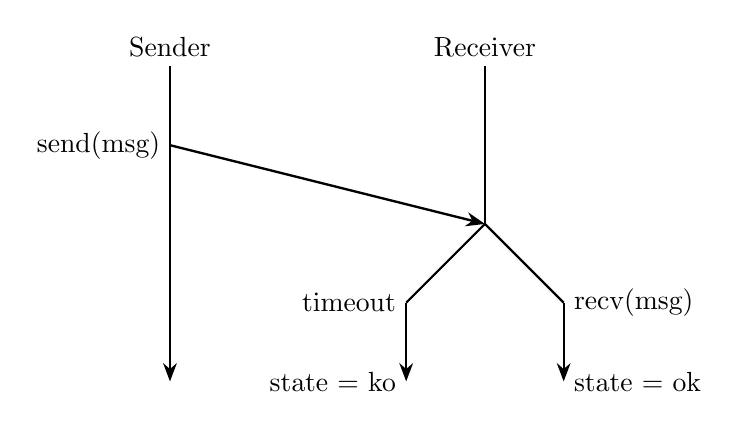
\begin{tikzpicture}[>=Stealth]
    % Draw the vertical lines for sender and receiver with arrowheads at the bottom
    \draw [thick, ->] (0,0) -- (0,-4) node[at start, above] {Sender};
    \draw [thick] (4,0) -- (4,-2) node[at start, above] {Receiver};

    % Label for send(msg) at sender's timeline
    \draw (0,-1) node[left] {send(msg)} node[right] {};

    % Draw the diagonal arrow from sender to receiver with a larger arrowhead
    \draw [->, line width=0.3mm] (0,-1) -- (4,-2);

    % Receiver line splits into two branches
    % Branch for recv(msg)
    \draw [thick] (4,-2) -- (5,-3) node[at end, right] {recv(msg)};
    \draw [thick, ->] (5,-3) -- (5,-4) node[at end, right] {state = ok};

    % Branch for timeout
    \draw [thick] (4,-2) -- (3,-3) node[at end, left] {timeout};
    \draw [thick, ->] (3,-3) -- (3,-4) node[at end, left] {state = ko};
\end{tikzpicture}

This setup illustrates the sender's action of sending a message and the receiver's subsequent state transition based on message receipt or timeout, demonstrating different outcomes in a distributed communication scenario.

\subsection{Interception of System Calls using LD\_PRELOAD}
The \texttt{redirect.c} file in the SimpleSendRecv directory implements the interception of system calls using the \texttt{LD\_PRELOAD} technique. This approach allows overriding standard library functions, such as \texttt{send} and \texttt{recv}, to redirect their execution to a controller process.

\subsubsection{Background on LD\_PRELOAD}
\texttt{LD\_PRELOAD} is an environment variable in Unix-like systems used to load user-defined shared libraries before standard ones. This technique enables function overriding without altering the original program's source code.

\subsubsection{Custom send and recv Functions}
The custom \texttt{send} and \texttt{recv} functions in \texttt{redirect.c} intercept calls to these standard functions. The \texttt{send} function establishes a connection with the controller and sends data, while the \texttt{recv} function handles data reception and initiates state exploration processes.

\begin{verbatim}
// Custom send function
ssize_t send(int sockfd, const void *buf, size_t len, int flags) {
    // ... (implementation details)
}

// Custom recv function
ssize_t recv(int sockfd, void *buf, size_t len, int flags) {
    // ... (implementation details)
}
\end{verbatim}

\subsubsection{Diagram of Process Interception}
The interception process can be visualized as follows:
\begin{verbatim}
[Application] --(send/recv)--> [Custom Function] --(redirect)--> [Controller]
\end{verbatim}

\subsection{Controller Process in SimpleSendRecv}
The \texttt{controller.c} file orchestrates the state space exploration process in the SimpleSendRecv component of the project.

\subsubsection{Process Management}
The controller spawns the sender and receiver processes and uses \texttt{LD\_PRELOAD} to intercept their communication:

\begin{verbatim}
// Spawning processes
processes[0] = spawn_process("process2"); // Receiver
sleep(3); // Ensure connection setup
processes[1] = spawn_process("process1"); // Sender
\end{verbatim}

\subsubsection{Interception and State Exploration}
The controller listens for intercepted messages and forks the receiver's execution to explore different states:

\begin{verbatim}
// Listen for incoming messages
while ((connfd = accept(sockfd, NULL, NULL)) != -1) {
    // ... (code to handle incoming messages)
    if (strncmp(buffer, "rec", 3) == 0) {
        // Handle receiver wanting to receive a message
        // ... (code to send message and explore states)
    }
    // ... (additional code for handling send messages and state exploration)
}
\end{verbatim}

\subsubsection{Diagram of Interaction and State Exploration}
The interaction between the sender, receiver, and controller, along with the state exploration process, can be visualized as follows:

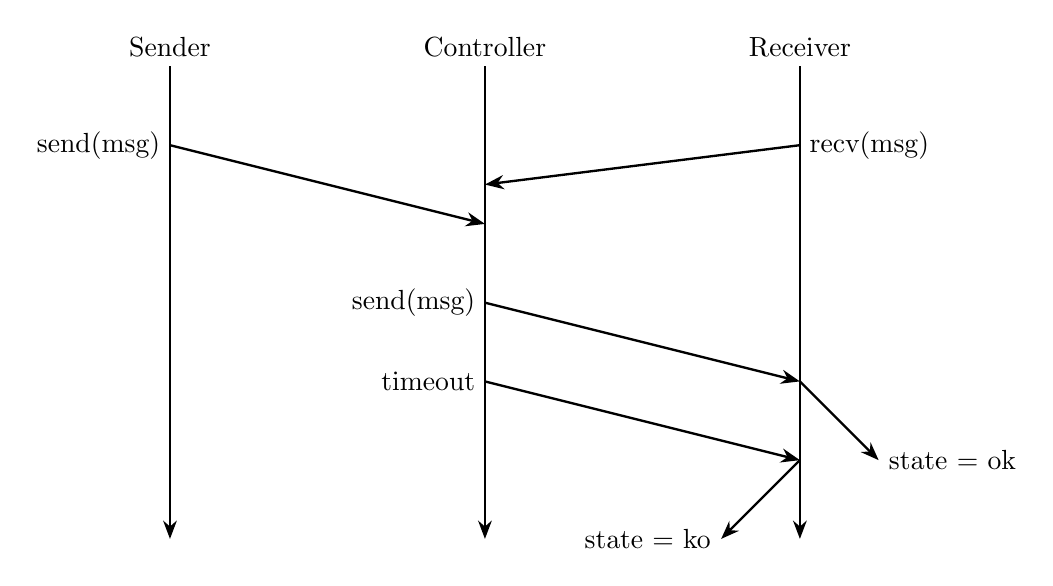
\begin{tikzpicture}[>=Stealth]
    % Draw the vertical lines for sender, receiver, and controller
    \draw [thick, ->] (0,0) -- (0,-6) node[at start, above] {Sender};
    \draw [thick, ->] (4,0) -- (4,-6) node[at start, above] {Controller};
    \draw [thick, ->] (8,0) -- (8,-6) node[at start, above] {Receiver};

    % Label for send(msg) at sender's timeline
    \draw (0,-1) node[left] {send(msg)} node[right] {};

    % Draw the arrow from sender to controller
    \draw [->, line width=0.3mm] (0,-1) -- (4,-2);

    % Label for recv(msg) at receiver's timeline
    \draw (8,-1) node[right] {recv(msg)} node[left] {};

    % Draw the arrow from receiver to controller
    \draw [->, line width=0.3mm] (8,-1) -- (4,-1.5);

    % Label for send(msg) at controller's timeline to receiver
    \draw (4,-3) node[left] {send(msg)} node[right] {};

    % Draw the arrow from controller to receiver
    \draw [->, line width=0.3mm] (4,-3) -- (8,-4);

    % Receiver line splits for recv(msg)
    \draw [thick, ->] (8,-4) -- (9,-5) node[at end, right] {state = ok};

    % Label for timeout at controller's timeline to receiver
    \draw (4,-4) node[left] {timeout} node[right] {};

    % Draw the arrow from controller to receiver for timeout
    \draw [->, line width=0.3mm] (4,-4) -- (8,-5);

    % Receiver main line splits for timeout
    \draw [thick, ->] (8,-5) -- (7,-6) node[at end, left] {state = ko};
\end{tikzpicture}

This setup demonstrates the first case of state space exploration in a distributed system using a central controller, highlighting the project's innovative approach to distributed system testing.

\subsection{BV-Broadcast and Byzantine BV-Broadcast Processes}
The \texttt{bv\_broadcast.c} and \texttt{byzantine\_bv\_broadcast.c} files implement the BV-broadcast algorithm and its Byzantine variant.

\subsubsection{bv\_broadcast.c}
This file contains the standard BV-broadcast algorithm:

\begin{verbatim}
void BV_broadcast(int value) {
    // ... (broadcast logic)
    send(sockfd, &message, sizeof(message), 0);
    // ... (additional logic)
}

void processMessages(int value, int fromProcess) {
    // ... (processing logic)
    if (distinctCount > T && !hasBroadcasted[value]) {
        BV_broadcast(value);
    }
    // ... (commit logic)
}
\end{verbatim}

\subsubsection{byzantine\_bv\_broadcast.c}
This file implements a Byzantine process with malicious behavior:

\begin{verbatim}
void malicious_BV_broadcast() {
    // ... (malicious broadcast logic)
    send(sockfd, &message, sizeof(message), 0);
    // ... (additional logic)
}
\end{verbatim}

\subsubsection{Diagram of BV-Broadcast Process}
The BV-broadcast process can be visualized as follows:
TODO nicer graph

\begin{verbatim}
[BV-Broadcast Process] --(broadcast)--> [Network]
                          |
                          |---(receive)--> [Process Messages]
                                            |
                                            |--(broadcast further/commit)--> [State Update]
\end{verbatim}

These implementations demonstrate the core functionality of the BV-broadcast algorithm and its adaptation for Byzantine behavior in distributed systems.

\subsection{BV-Controller Process}
The \texttt{bvcontroller.c} file is responsible for managing the execution of the BV-broadcast processes in the project.

\subsubsection{Functionality}
The controller creates a semaphore for synchronization and spawns child processes for each instance of the BV-broadcast algorithm. It then executes the appropriate version of the BV-broadcast process:

\begin{verbatim}
int main() {
    // ... (semaphore creation and process spawning code)
    for (int i = 0; i < N; i++) {
        if ((child_pids[i] = fork()) == 0) {
            // ... (code to execute BV-broadcast or Byzantine BV-broadcast)
        }
    }
    // ... (code to signal and wait for child processes)
}
\end{verbatim}

This controller plays a pivotal role in orchestrating the execution of both standard and Byzantine variants of the BV-broadcast algorithm, ensuring the proper functioning of the distributed system.

\subsection{System State in BV-Broadcast}
In the BV-broadcast algorithm, the state of each process is represented as a duplet \((count\_0, count\_1)\), indicating the counts of received values 0 and 1. The system state is a collection of these duplets from all participating processes.

\subsection{Diamond Problem in BV-Broadcast}
The diamond problem in the BV-broadcast algorithm is illustrated using a specific example, demonstrating how different event sequences can lead to the same system state.

\subsubsection{Initial Setup and State Exploration}
Initially, four processes have values 0, leading to the state \(((1,0), (1,0), (1,0), (1,0))\). Process 1 sends a message to Process 0, and we consider both values 0 and 1, forking Process 0 for each scenario.

\subsubsection{Resulting State}
Further message reception in both scenarios leads to the same state \(((2,1), (1,0), (1,0), (1,0)\), exemplifying the diamond problem. This convergence allows for optimization in state space exploration by eliminating redundant paths.

\subsubsection{Visualization}
\begin{verbatim}
Initial State: ((1,0), (1,0), (1,0), (1,0))

        Process 1 sends value to Process 0
                  /                 \
                 /                   \
                0                     1
               /                       \
              /                         \
((2,0), (1,0), (1,0), (1,0))   ((1,1), (1,0), (1,0), (1,0))
              \                         /
               \                       /
                Process 2 sends value to Process 0
                (0 in first, 1 in second scenario)
                 \                     /
                  \                   /
                   \                 /
                ((2,1), (1,0), (1,0), (1,0))
\end{verbatim}

This example demonstrates the efficiency of the state space exploration process in the BV-broadcast algorithm by addressing the diamond problem.

\subsection{Identifying Invalid States in BV-Broadcast}
The program checks each property of the BV-broadcast algorithm to identify invalid states, using the system state representation.

\subsubsection{BV-Obligation}
The program verifies that if \( t+1 \) or more processes broadcast a value, it must be present in every correct process's state. An invalid state is flagged if this condition is not met.

The program verifies the BV-Obligation property in the BV-broadcast algorithm using the system state representation.

\subsubsection{Broadcast Criteria for Correct Processes}
A value is considered broadcasted by a correct process if it is the process's initial value or if the process received the value in at least \( T + 1 \) messages from different processes.

\subsubsection{Verification Process}
\begin{enumerate}
    \item \textbf{Identify Broadcasted Values:} The program determines values broadcasted by more than \( T \) correct processes by analyzing initial values and received value counts in each process's state.
    \item \textbf{Check Commitment by Correct Processes:} For each identified value, the program verifies if it has been received more than \( 2 \times T \) times by every correct process, indicating commitment.
    \item \textbf{Property Validation:} The BV-Obligation property is upheld if all values broadcasted by more than \( T \) correct processes are committed by all correct processes. The program identifies any state and execution path where this property fails.
\end{enumerate}

\subsubsection{BV-Justification}
The program ensures that any value in a correct process's state must have been broadcast by at least one correct process. An invalid state occurs if a value cannot be traced back to a correct process's broadcast.

\subsection{Verifying BV-Justification in BV-Broadcast}
The program verifies the BV-Justification property in the BV-broadcast algorithm using the system state representation.

\subsubsection{Commitment Criteria}
A value is considered committed by a correct process if it has been received from more than \( 2 \times T \) different processes, as determined by examining the process's state.

\subsubsection{Broadcast Criteria for Correct Processes}
A value is broadcasted by a correct process if it is the process's initial value or if it was received from more than \( T \) different processes.

\subsubsection{Verification Process}
\begin{enumerate}
    \item \textbf{Identify Committed Values:} The program determines committed values by checking if they have been received from more than \( 2 \times T \) different processes.
    \item \textbf{Validate Broadcast by Correct Processes:} For each committed value, the program verifies that it has been broadcasted by a correct process.
    \item \textbf{Property Validation:} The BV-Justification property is upheld if all values committed by correct processes have been broadcasted by correct processes. The program identifies any state and execution path where this property fails.
\end{enumerate}


\subsubsection{BV-Uniformity}
The program checks for consistency in the presence of a value across the states of all correct processes. An invalid state is identified if there is inconsistency in value presence.

\subsection{Verifying BV-Uniformity in BV-Broadcast}
The program verifies the BV-Uniformity property in the BV-broadcast algorithm using the system state representation.

\subsubsection{Commitment Criteria}
A value is considered committed by a correct process if it has been received from more than \( 2 \times T \) different processes.

\subsubsection{Verification Process}
\begin{enumerate}
    \item \textbf{Identify Committed Values:} The program determines committed values for each correct process by examining their states.
    \item \textbf{Check Uniformity Across Correct Processes:} For each committed value, the program verifies that it is also committed by every other correct process.
    \item \textbf{Property Validation:} The BV-Uniformity property is upheld if every value committed by one correct process is also committed by all other correct processes. The program identifies any state and execution path where this property fails.
\end{enumerate}


\subsubsection{BV-Termination}
The program verifies that each correct process's state eventually includes at least one value. An invalid state is flagged if any correct process's state remains empty beyond a certain execution point.

\subsection{Verifying BV-Termination in BV-Broadcast}
The program verifies the BV-Termination property in the BV-broadcast algorithm using the system state representation.

\subsubsection{Commitment Criteria}
A value is considered committed by a correct process if it has been received from more than \( 2 \times T \) different processes.

\subsubsection{Verification Process}
\begin{enumerate}
    \item \textbf{Check for Committed Values:} The program verifies for each correct process whether it has committed at least one value by checking their states.
    \item \textbf{Property Validation:} The BV-Termination property is upheld if every correct process has committed at least one value. The program identifies any state where this property fails.
\end{enumerate}

\subsection{Process of Verifying BV-Broadcast Properties}
The program conducts a thorough verification of the BV-broadcast properties for each system state individually and then across all states to ensure the integrity of the algorithm.

\subsubsection{Individual State Verification}
For each system state, the program verifies the BV-Obligation, BV-Justification, BV-Uniformity, and BV-Termination properties. If any property fails, the state is flagged as invalid.

\subsubsection{Comprehensive System State Verification}
The verification process is repeated for each state in the system. The program identifies any invalid states and uses the controller's information to trace the initial state and the specific messages that led to these states.

\subsubsection{Property Validation and Traceability}
This approach ensures the overall correctness of the BV-broadcast algorithm. Identifying invalid states and their corresponding execution paths provides valuable insights into potential issues or vulnerabilities in the algorithm or its implementation.

\subsection{State Space Exploration Process in BV-Broadcast}
The state space exploration process in the BV-broadcast algorithm involves forking process executions upon message reception and systematically updating the system state representation in the controller.

\subsubsection{Execution and Forking}
Each process executes as per the system design. Upon message reception, the controller forks the process execution, with each child process continuing with specific values to represent different scenarios.

\subsubsection{State Representation Update}
The controller updates its representation of the system states by duplicating and modifying them for each forked process. This ensures that all possible outcomes of message reception are covered without excessive parallel executions.

\subsubsection{Efficient Exploration}
This approach allows for efficient and comprehensive coverage of the state space, ensuring thorough testing and validation of the algorithm. The controller's methodical tracking of all possible system states enhances the effectiveness of the state space exploration process.

\subsection{Functionality of redirect.c in BV-Broadcast}
The \texttt{redirect.c} file in the BvBroadcast directory implements the interception and redirection of system calls in the BV-broadcast algorithm.
It plays a pivotal role in controlling the message flow in the BV-broadcast algorithm, crucial for state space exploration.
The overridden \texttt{send} and \texttt{recv} functions allow the communication between BV-broadcast processes and the controller:

\subsubsection{Overridden send Function}
The custom \texttt{send} function serves two primary purposes:
\begin{enumerate}
    \item \textbf{Differentiating Message Types:} It distinguishes between initial broadcast messages and echo messages, essential for simulating the BV-broadcast behavior accurately.
    \item \textbf{Feedback Channel:} When \texttt{sockfd} is -1, the function acts as a feedback channel, allowing processes to communicate their state changes to the controller.
\end{enumerate}

\begin{verbatim}
// Overridden send function
ssize_t send(int sockfd, const void *buf, size_t len, int flags) {
    // ... (implementation details)
}
\end{verbatim}

\subsubsection{Overridden recv Function}
The custom \texttt{recv} function is instrumental in the state exploration process:
\begin{enumerate}
    \item \textbf{Indicating Readiness to Receive:} It notifies the controller when a process is ready to receive a message, crucial for decision-making in state exploration.
    \item \textbf{Waiting for Instructions:} The process waits for the controller's instructions, which may involve forking the process execution to explore different scenarios.
\end{enumerate}

\begin{verbatim}
// Overridden recv function
ssize_t recv(int sockfd, void *buf, size_t len, int flags) {
    // ... (implementation details)
}
\end{verbatim}

TODO for all the small sections add code snippet ?
\subsection{Controller Process in BV-Broadcast}
The \texttt{controller.c} file is central to the state space exploration in the BV-Broadcast algorithm, orchestrating the entire process from process management to state exploration.

\subsubsection{Process Management}
The controller is responsible for spawning and managing the execution of BV-broadcast processes, ensuring controlled and sequential execution for accurate state space exploration.

\begin{verbatim}
void spawnProcesses() {
    // ... (process spawning and execution control logic)
}
\end{verbatim}

\subsubsection{Message Handling and Matching}
The controller adeptly handles and matches intercepted messages, ensuring they reach their intended destinations and accurately simulating distributed system communication.

\subsubsection{State Exploration for Byzantine Processes}
For Byzantine processes, the controller initiates state exploration by forking the receiver process and exploring both possible states (receiving 0 or 1), crucial for understanding the impact of Byzantine behavior.

\subsubsection{State Recovery and Comparison}
After processing a message, the controller recovers the receiver's state and compares it with existing states, identifying and eliminating redundant states to optimize the exploration process.

\subsubsection{Elimination of Redundant States}
The elimination of redundant states is a key functionality of the controller, ensuring that the exploration process remains efficient and focused only on unique and relevant states.



\subsubsection{Diagrams of Process Interaction and State Exploration}
The interaction between the controller and BV-broadcast processes, along with the state exploration process, can be visualized as follows:


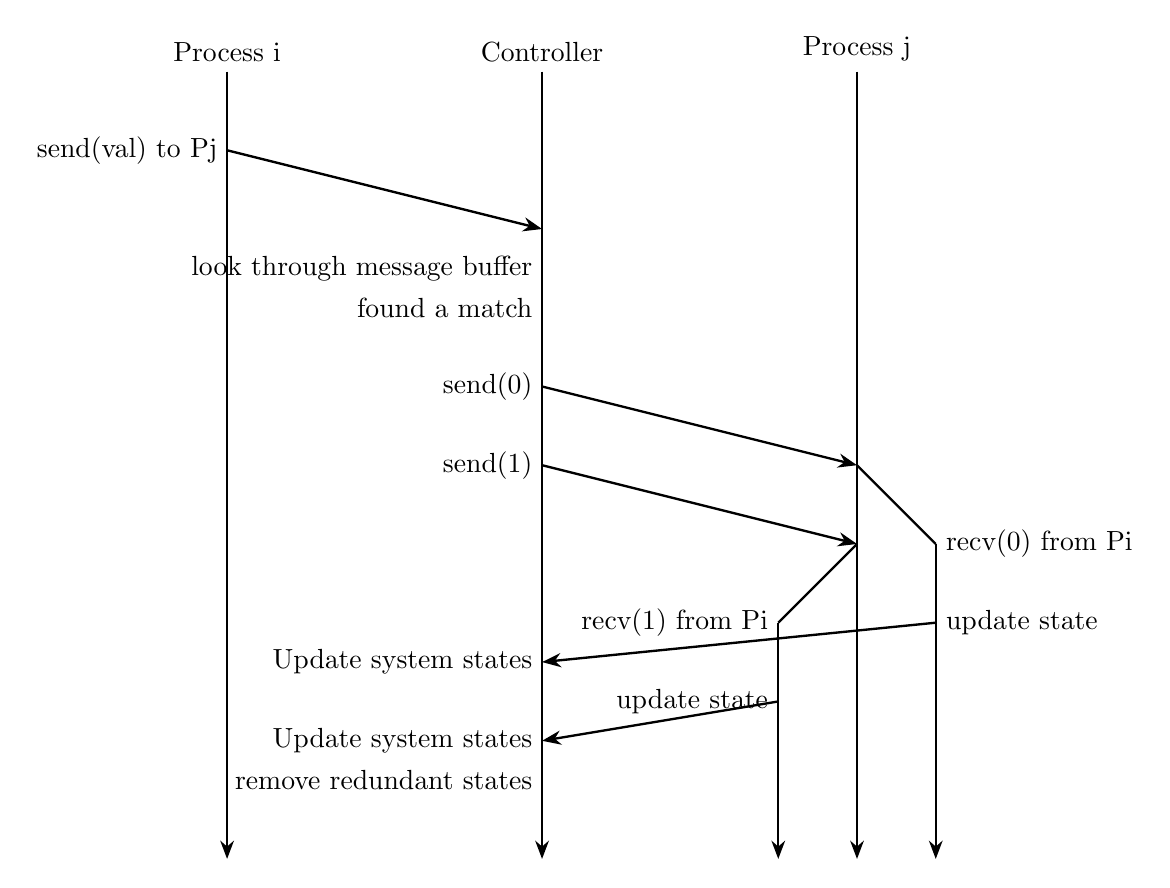
\begin{tikzpicture}[>=Stealth]
    % Draw the vertical lines for Process i, Process j, and Controller
    \draw [thick, ->] (0,0) -- (0,-10) node[at start, above] {Process i};
    \draw [thick, ->] (4,0) -- (4,-10) node[at start, above] {Controller};
    \draw [thick, ->] (8,0) -- (8,-10) node[at start, above] {Process j};

    % Label for send(val) at Process i's timeline
    \draw (0,-1) node[left] {send(val) to Pj} node[right] {};

    % Draw the arrow from Process i to Controller
    \draw [->, line width=0.3mm] (0,-1) -- (4,-2);

    % Controller processes the message
    \draw (4,-2.5) node[left] {look through message buffer} node[right] {};
    \draw (4,-3) node[left] {found a match} node[right] {};

    % Label for send(0) at Controller's timeline to Process j
    \draw (4,-4) node[left] {send(0)} node[right] {};

    % Draw the arrow from Controller to Process j for send(0)
    \draw [->, line width=0.3mm] (4,-4) -- (8,-5);

    % Process j line splits for recv(0)
    \draw [thick] (8,-5) -- (9,-6) node[at end, right] {recv(0) from Pi};
    \draw [thick] (9,-6) -- (9,-7) node[at end, right] {update state};
    \draw [->, line width=0.3mm] (9,-7) -- (4,-7.5); % Arrow back to Controller
    \draw [thick, ->] (9,-7) -- (9,-10); % Continue branch downwards

    % Label for send(1) at Controller's timeline to Process j
    \draw (4,-5) node[left] {send(1)} node[right] {};

    % Draw the arrow from Controller to Process j for send(1)
    \draw [->, line width=0.3mm] (4,-5) -- (8,-6);

    % Process j main line splits for recv(1)
    \draw [thick] (8,-6) -- (7,-7) node[at end, left] {recv(1) from Pi};
    \draw [thick] (7,-7) -- (7,-8) node[at end, left] {update state};
    \draw [->, line width=0.3mm] (7,-8) -- (4,-8.5); % Arrow back to Controller
    \draw [thick, ->] (7,-8) -- (7,-10); % Continue branch downwards

    % Controller updates system states
    \draw (4,-7.5) node[left] {Update system states} node[right] {};
    \draw (4,-8.5) node[left] {Update system states} node[right] {};
    \draw (4,-9) node[left] {remove redundant states} node[right] {};
\end{tikzpicture}

This setup demonstrates the sophisticated state space exploration capabilities in the BV-broadcast algorithm using a central controller, highlighting the project's advanced approach to distributed system testing.


\subsection{Development of the State Space Exploration Tool}
The state space exploration tool was initially designed with a focus on simplicity, targeting basic send-receive operations. This foundational design was crucial for ensuring the tool's adaptability and scalability. As the project evolved, the tool was extended to accommodate the more complex bv broadcast algorithm. 

This progression from a simple send-receive model to a more sophisticated broadcast algorithm exemplifies the tool's flexible architecture. The design challenges involved in this transition were significant, particularly in ensuring that the tool remained efficient and effective when dealing with more complex algorithms. This adaptability is a testament to the robust and modular design of the tool, allowing for future extensions to other distributed algorithms.


??????
\subsection{Influence of the Shadow Project}
The initial exploration of integrating with the Shadow project provided valuable insights, despite the eventual decision to develop an independent tool. The experience with Shadow highlighted the complexities of working with an existing, production-level system and influenced the design decisions for our tool. 

This experience underscored the need for a more tailored solution that could be more closely aligned with the specific goals of our project. It also provided a clear understanding of the features and capabilities required for effective state space exploration in distributed systems, which were then incorporated into the design of our own tool.


\subsection{Overall Design Cohesion}
The design of the project is a cohesive blend of algorithmic precision and flexible tool architecture. Each component, from the broadcast algorithm to the state space exploration tool, is intricately linked to the overarching goal of enhancing reliability and fault tolerance in distributed systems. 

This cohesive design ensures that the tool not only addresses the immediate needs of testing and validating the bv broadcast algorithm but is also equipped to handle future challenges and extensions to other distributed algorithms. The project's design is a reflection of a deep understanding of the complexities of distributed systems and a commitment to developing solutions that are both robust and adaptable.



%%%%%%%%%%%%%%%%%%%%%%%%
\chapter{Implementation}
%%%%%%%%%%%%%%%%%%%%%%%%

\section{Instructions / advice}
The implementation covers some of the implementation details of your project.
This is not intended to be a low level description of every line of code that
you wrote but covers the implementation aspects of the projects.

This section is usually 3-5 pages.

\section{Actual text}




%%%%%%%%%%%%%%%%%%%%
\chapter{Evaluation}
%%%%%%%%%%%%%%%%%%%%

\section{Instructions / advice}
In the evaluation you convince the reader that your design works as intended.
Describe the evaluation setup, the designed experiments, and how the
experiments showcase the individual points you want to prove.

This section is usually 5-10 pages.

\section{Actual text}

\subsection{State Space Reduction through Centralized Control}
One of the key metrics for evaluating the effectiveness of the state space exploration tool is its ability to reduce the number of states that need to be explored. By leveraging a central controller, the tool can identify and eliminate redundant states early in the exploration process. This approach significantly streamlines the testing procedure, making it more efficient and less resource-intensive. A quantitative analysis of the number of states eliminated provides a clear measure of the tool's efficiency. This section should detail the specific methods used to identify redundant states and the extent to which state exploration was reduced in both the simple send-receive and bv broadcast algorithms.

\subsection{Bug Introduction and Detection in bv Broadcast}
TODO add specific examples
Another critical aspect of the evaluation involves introducing bugs into the bv broadcast algorithm and assessing the tool's ability to reach and identify invalid states. This process not only tests the robustness of the bv broadcast algorithm itself but also demonstrates the tool's capability in uncovering potential vulnerabilities. 

\subsection{Implications of Findings}
The results of these evaluations have significant implications for the field of distributed system testing. The ability to efficiently reduce state space and accurately detect bugs addresses two of the most pressing challenges in the field. Discuss how these findings contribute to the broader goals of improving the reliability and security of distributed systems. Reflect on the potential impact of this tool in real-world scenarios, particularly in systems where fault tolerance and security are critical.

\subsection{Conclusion}
Conclude the evaluation section by summarizing the key findings and their significance. Emphasize the novel contributions of your tool in the context of distributed system testing and its potential applications in various domains. This section should reinforce the value of your research and set the stage for future work that can build upon these findings.

\section{Evaluation of State Space Exploration in BV-Broadcast}
The evaluation of the state space exploration process in the BV-broadcast algorithm demonstrates the program's effectiveness in identifying invalid states and its efficiency in reducing the state space.

\subsection{Identification of Invalid States}
The program successfully identified invalid states in buggy implementations of the BV-broadcast algorithm, particularly those breaking the BV-Uniformity property. Detailed examples and results will be provided to illustrate these findings.

\subsection{State Space Reduction}
In a scenario with 3 processes, each sending 4 messages with 2 possible values, the program showed remarkable efficiency in state space exploration:

\begin{itemize}
    \item \textbf{Processed States:} The program navigated through 256 distinct system states.
    \item \textbf{States Killed:} A total of 135 redundant states were eliminated from the exploration process.
    \item \textbf{Total Potential States:} The theoretical total number of states for this scenario is \(2^{12} = 4096\).
\end{itemize}

These results indicate the program's effective approach to state space reduction, significantly decreasing the number of states that need to be explored for thorough testing and validation of the algorithm.

\section{Expanded Evaluation of State Space Exploration}
The expanded evaluation of the state space exploration process provides a comprehensive assessment of the program's capabilities across various scenarios and algorithms.

\subsection{Diverse Scenarios and Correct Implementations}
The program consistently identified no invalid states in correct implementations of the BV-broadcast algorithm, affirming its precision. Detailed examples of specific invalid states in buggy implementations will be provided.

\subsection{Testing with Various Numbers of Processes}
Testing with a varying number of processes, including scenarios with more than four processes, demonstrated the scalability of the program. The efficiency of state space exploration in these scenarios will be detailed, comparing explored versus theoretical state counts.

\subsection{Incorporating Additional Algorithms}
The application of the state space exploration tool to other algorithms, both fault-tolerant and non-fault-tolerant, will be discussed to showcase its versatility.

\subsection{Future Work and Improvements}
Potential areas for future research and development, such as optimization strategies, addition of more complex algorithms, and user interface enhancements, will be outlined.



%%%%%%%%%%%%%%%%%%%%%%
\chapter{Related Work}
%%%%%%%%%%%%%%%%%%%%%%

\section{Instructions / advice}
The related work section covers closely related work. Here you can highlight
the related work, how it solved the problem, and why it solved a different
problem. Do not play down the importance of related work, all of these
systems have been published and evaluated! Say what is different and how
you overcome some of the weaknesses of related work by discussing the 
trade-offs. Stay positive!

This section is usually 3-5 pages.

Discuss existing work in Byzantine fault-tolerant broadcast algorithms. Compare and contrast your approach with these works, highlighting what sets your project apart.

Review existing literature on distributed system testing, particularly focusing on state space exploration techniques. Compare your approach with existing methods, highlighting the novel aspects of your work.

Review existing literature on state space exploration tools in distributed systems. Compare your approach with existing methods, highlighting the unique aspects and adaptability of your tool.

\section{Actual text}

\subsection{Byzantine Fault-Tolerant Broadcast Algorithms}
The realm of Byzantine fault-tolerant (BFT) broadcast algorithms is rich with diverse approaches, each addressing the challenges of reliable communication in the presence of Byzantine faults. Renowned works in this domain, such as Castro and Liskov's Practical Byzantine Fault Tolerance (PBFT) and Kotla et al.'s Zyzzyva, have set significant benchmarks in ensuring system reliability and security. 

Our approach to BFT broadcasting, particularly through the bv broadcast algorithm, distinguishes itself by its simplicity and efficiency. Unlike PBFT, which requires a complex three-phase protocol for consensus, our bv broadcast algorithm achieves reliable communication with minimal overhead, making it more suitable for systems where resource efficiency is paramount. Furthermore, our approach addresses some of the scalability issues seen in traditional BFT algorithms, offering a more streamlined solution for modern distributed systems.

\subsection{State Space Exploration in Distributed System Testing}
State space exploration is a critical technique in distributed system testing, allowing researchers to understand the various possible states a system can encounter during its operation. Notable works in this area include Godefroid's model checking approach and Musuvathi et al.'s systematic testing method for finding heisenbugs in distributed systems.

Our project contributes to this field by introducing a novel approach that combines network emulation with process forking, enabling a more granular and controlled exploration of state spaces. This method allows for a more systematic and thorough testing process compared to existing techniques, which often rely on less controlled environment simulations or require extensive modifications to the tested systems.

\subsection{Tools for State Space Exploration in Distributed Systems}
The development of tools for state space exploration in distributed systems has been an area of active research, with tools like Microsoft's CHESS and the Java PathFinder being notable examples. These tools have been instrumental in advancing the field, providing frameworks for detecting concurrency errors and other issues in distributed systems.

Our tool sets itself apart through its adaptability and scalability. Unlike many existing tools that are often tailored to specific types of systems or algorithms, our tool is designed to be flexible, capable of handling a variety of distributed algorithms ranging from simple send-receive models to more complex broadcast algorithms. This adaptability makes it a valuable asset for a broader range of applications in distributed system testing.

\subsection{Conclusion}
In summary, while the related work in each of these domains has significantly advanced the field of distributed systems, our project introduces novel approaches and tools that address some of the limitations and challenges present in existing methods. By focusing on simplicity, efficiency, and adaptability, our work contributes meaningful advancements to the fields of Byzantine fault-tolerant broadcasting and state space exploration in distributed system testing.

\section{Comparative Analysis of Distributed System Testing Approaches}

\subsection{Grey-Box Fuzzing in Distributed Systems}
The recent development of Mallory, a framework for grey-box fuzz-testing of distributed systems, represents a significant advancement in the field. Unlike traditional black-box tools, which do not utilize past system behaviors to guide bug searches, Mallory adopts an adaptive approach. It employs a novel metric to maximize the observation of system behaviors by varying sequences of faults, thereby increasing the likelihood of uncovering new bugs. This method, which dynamically constructs and abstracts Lamport timelines of system behavior, represents a shift towards more intelligent and targeted testing strategies in distributed systems.

\subsection{Comparison with the Current Approach}
In contrast to Mallory's grey-box fuzzing, which aims to explore a large number of distinct states without attempting to cover every possible state, the approach in this thesis focuses on exhaustive state space exploration using a central controller. This method addresses the 'state space explosion problem' by eliminating redundant states early in the exploration process, effectively allowing for a comprehensive analysis of all potential system states. While both approaches aim to enhance the reliability and security of distributed systems, they differ in their strategies and focus areas.

\subsection{Relevance of Automated Testing and Bug Discovery}
The success of Mallory in discovering a significant number of zero-day bugs, including new vulnerabilities in well-tested systems like Braft, Dqlite, and Redis, underscores the critical importance of automated testing in distributed systems. This finding highlights the potential of both Mallory's grey-box fuzzing approach and the exhaustive state space exploration method presented in this thesis. Automated testing not only aids in identifying potential system faults and vulnerabilities but also plays a crucial role in enhancing the overall security and robustness of distributed systems.

\section{Conclusion}
The comparison with Mallory's approach and the discussion on the relevance of automated testing in distributed systems provide a broader context for this thesis. It demonstrates the diverse methodologies being developed to tackle the complexities of distributed system testing and highlights the significant contributions of this work in advancing the field.

\section{Testing Methodologies in Distributed Systems}

\subsection{Black Box vs Grey Box vs White Box Testing}
In the realm of distributed system testing, methodologies can be broadly categorized into black box, grey box, and white box testing. Black box testing, exemplified by tools like Jepsen, does not rely on internal knowledge of the system's workings and tests the system from an external perspective. Grey box testing, as employed by Mallory, strikes a balance between black box and white box testing. It leverages some knowledge of the system's internal state or structure but does not require full access, thereby guiding the testing process more effectively than black box methods. For instance, Mallory's grey box approach enables it to explore 54.27% more states than Jepsen's black box method.

\subsection{Exhaustive State Space Exploration: A White Box Approach}
Contrasting with these methods, the approach in this thesis aligns more closely with white box testing. It involves exhaustive exploration of the state space, leveraging complete knowledge of the system's internal workings. By using a central controller to simulate the execution of the distributed system, this method systematically explores all possible states, effectively addressing the 'state space explosion problem' and ensuring comprehensive coverage. This exhaustive exploration is a significant departure from both black box and grey box methods, which only explore a subset of possible states.

\subsection{Significance of Complete State Exploration}
The ability to explore all possible states in a distributed system is particularly noteworthy. While grey box methods like Mallory show a marked improvement over black box methods in terms of state exploration and bug discovery, the exhaustive approach of this thesis ensures that no potential state or behavior is overlooked. This comprehensive coverage is crucial for identifying and rectifying all possible faults and vulnerabilities, significantly enhancing the reliability and security of distributed systems.

\section{Conclusion}
This discussion on different testing methodologies highlights the unique position of this thesis in the landscape of distributed system testing. By adopting an approach akin to white box testing, this work sets a new standard in terms of thoroughness and reliability, offering a more complete solution to the challenges of distributed system testing.



%%%%%%%%%%%%%%%%%%%%
\chapter{Conclusion}
%%%%%%%%%%%%%%%%%%%%

\section{Instructions / advice}
In the conclusion you repeat the main result and finalize the discussion of
your project. Mention the core results and why as well as how your system
advances the status quo.

Summarize the key findings of your research, particularly the effectiveness of network emulation and process forking in exploring the state space of distributed systems. Discuss the implications of your findings for the testing of distributed systems and potential areas for future research.

Reflect on the broader impact of your work. Reiterate the importance of robust testing in distributed systems, given their widespread use and the severe implications of bugs leading to cyber threats. Discuss how your tool represents a step forward in preemptive security measures, potentially aiding in the early detection and prevention of zero-day attacks and other vulnerabilities. Conclude with thoughts on how your work contributes to the field of distributed systems and cybersecurity, and suggest directions for future research that could build upon your findings.

Summarize the key findings of your research, particularly the development and validation of a versatile state space exploration tool for distributed systems. Discuss the implications of your findings for the testing and reliability of distributed systems, and the potential for extending the tool to other complex algorithms. Conclude with thoughts on future research directions and improvements to the tool.

Reflect on the entire journey of the project, including the initial exploration with Shadow. Discuss how these early challenges shaped the direction and outcomes of your project.

\section{Actual text}

\subsection{Summary of Key Findings}
This thesis presented a comprehensive exploration into the state space of distributed systems, leveraging network emulation and process forking techniques. The core result of this research is the successful development and validation of a versatile tool for state space exploration, capable of adapting to various distributed algorithms. This tool represents a significant advancement in the testing and reliability of distributed systems, particularly in its ability to handle complex scenarios like Byzantine fault-tolerant broadcast algorithms.

\subsection{Implications and Future Research}
The implications of this research are far-reaching, especially in the context of distributed systems' testing. The ability to systematically explore state spaces and identify potential faults or vulnerabilities preemptively is crucial, given the increasing reliance on distributed systems in critical domains. This tool not only enhances our understanding of these systems but also opens up new avenues for future research, particularly in extending its capabilities to more complex algorithms and scenarios.

Moreover, the broader impact of this work in the realm of cybersecurity cannot be overstated. In an era where cyber threats are increasingly sophisticated, the early detection and prevention of vulnerabilities, including zero-day attacks, are paramount. This project contributes significantly to these efforts, offering a new tool in the arsenal against such threats.

\subsection{Reflections on the Project Journey}
Reflecting on the journey of this project, the initial exploration with the Shadow emulator was a pivotal phase. Although it did not culminate in direct integration, this early exploration was instrumental in shaping the direction and outcomes of the research. It highlighted the complexities and challenges inherent in distributed system testing and underscored the need for a more adaptable and efficient approach, which this project successfully developed.

\subsection{Concluding Thoughts}
In conclusion, this thesis not only contributes a novel tool to the field of distributed systems but also advances our understanding of how to effectively test and secure these complex systems. The journey from conceptualization to realization underscores the dynamic nature of research and development in this field. Future research, building upon these findings, has the potential to further revolutionize our approach to ensuring the reliability and security of distributed systems.


\cleardoublepage
\phantomsection
\addcontentsline{toc}{chapter}{Bibliography}
\printbibliography

% Appendices are optional
% \appendix
% %%%%%%%%%%%%%%%%%%%%%%%%%%%%%%%%%%%%%%
% \chapter{How to make a transmogrifier}
% %%%%%%%%%%%%%%%%%%%%%%%%%%%%%%%%%%%%%%
%
% In case you ever need an (optional) appendix.
%
% You need the following items:
% \begin{itemize}
% \item A box
% \item Crayons
% \item A self-aware 5-year old
% \end{itemize}

\end{document}